\chapter{Metodologia}
\label{chap:metodologia}
As informações a seguir detalham as etapas da metodologia utilizada para a condução deste estudo. Sendo elas: o delineamento da pesquisa, a origem e natureza dos dados, os métodos de coleta e tratamento dos dados, os procedimentos de pré-processamento e agregação, a engenharia de variáveis desenvolvida para aprofundar a análise e, por fim, as técnicas de estatística inferencial empregadas para testar hipóteses e construir um modelo preditivo. Cada etapa é descrita com o objetivo de garantir a transparência e a replicabilidade do estudo. Além de especificar softwares e bibliotecas utilizadas.

\begin{figure}[h!]
    \centering
    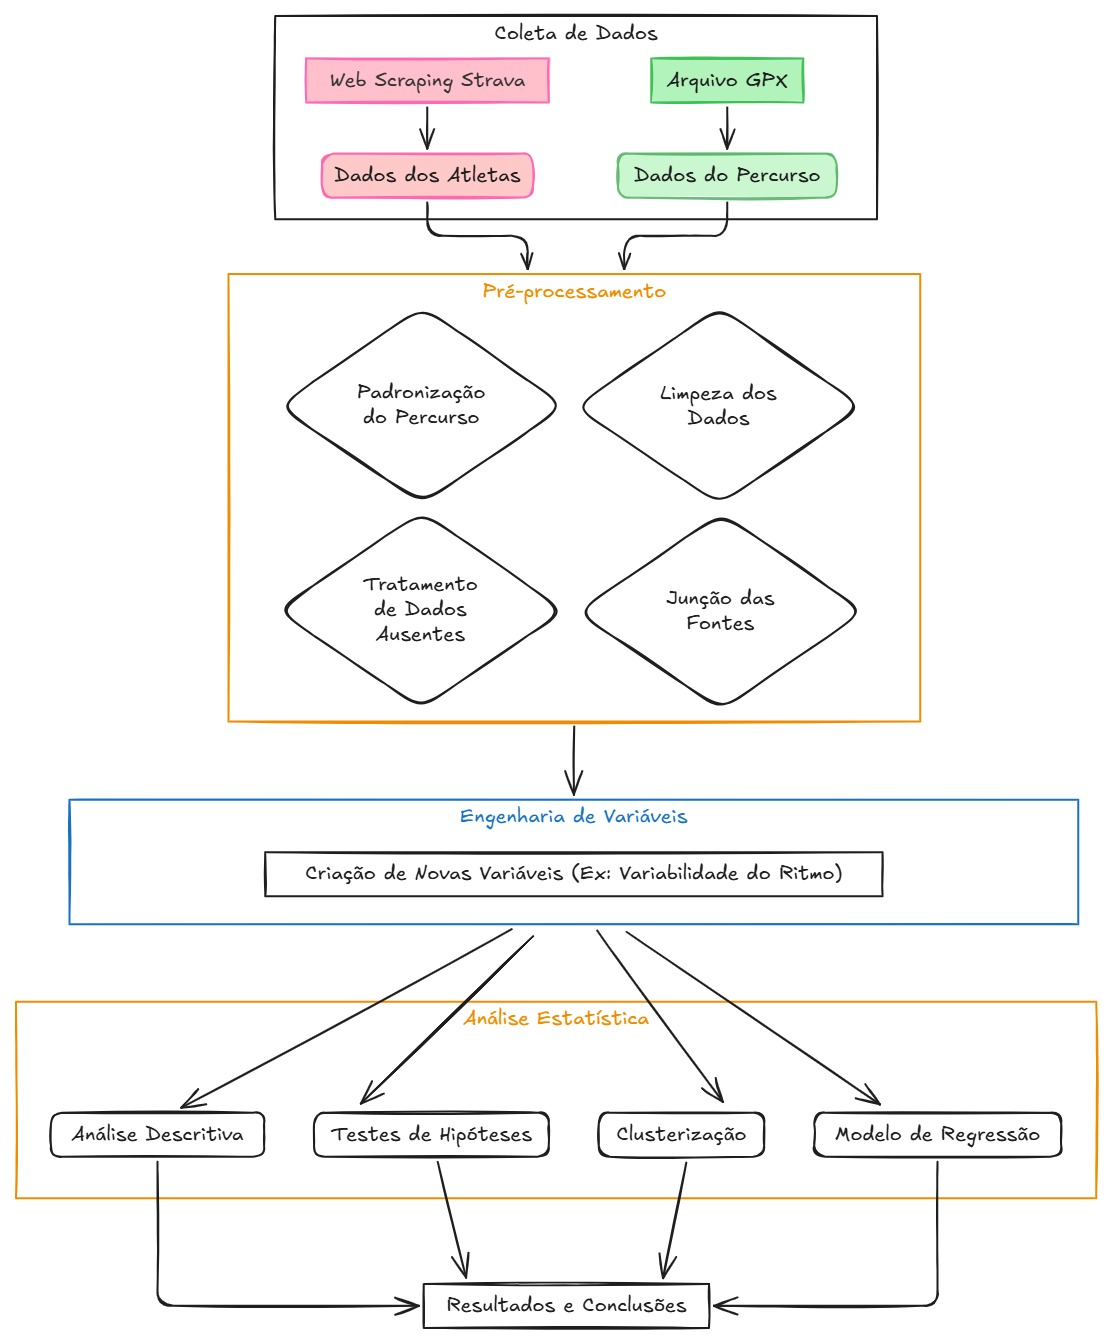
\includegraphics[width=0.75\textwidth]{Imagens/fluxo_trabalho.png}
    \caption{Fluxograma do processo de coleta e análise de dados. Fonte: Elaborado pelo autor (2025).}
    \label{fig:fluxograma}
\end{figure}

\section{Delineamento da Pesquisa}

Foi realizado um estudo quantitativo, de caráter descritivo e explicativo. Descritivo por meio da Análise Exploratória de Dados (AED), que visa caracterizar o perfil dos atletas da amostra. Explicativo ao utilizar técnicas de estatística inferencial, como a regressão linear múltipla, para modelar e explicar a relação entre um conjunto de variáveis e o desempenho final dos corredores.

\section{Fonte e Natureza dos Dados}
\label{sec:fonte_dados}

Os dados utilizados neste estudo foram extraídos da plataforma de rastreamento de atividades físicas Strava, referentes às edições de 2022 e 2023 da prova de \emph{trekking} de montanha \textit{La Misión Brasil}, na modalidade de 35 quilômetros. A extração foi realizada por meio de técnicas de \emph{web scraping}, conforme detalhado na Seção \ref{subsec:scraping}.

A natureza do conjunto de dados original era granular, com cada linha representando o desempenho de um único atleta em um quilômetro específico da prova. Essa estrutura, embora detalhada, não era adequada para uma análise centrada no desempenho geral do atleta, necessitando de uma etapa de agregação.

\section{Coleta e Pré-processamento dos Dados}

A obtenção dos dados foi dividida em quatro fases principais: padronização das informações do percurso, extração automatizada de dados da web, limpeza e estruturação final do conjunto de dados.

\subsection{Padronização dos Dados do Percurso via GPX}
\label{subsec:gpx}

A fim de garantir a consistência e a padronização das variáveis geográficas do percurso para todos os atletas, evitando discrepâncias inerentes a diferentes dispositivos de GPS, o ponto de partida foi a análise de um arquivo GPX (GPS Exchange Format) oficial da prova. Este arquivo foi processado para extrair informações de elevação a cada quilômetro, criando um gabarito do percurso com 36 segmentos. Essa abordagem permitiu que variáveis como ganho de elevação positivo e negativo de um determinado quilômetro fossem padronizadas e atribuídas de forma idêntica a todos os corredores da amostra.

\subsection{Extração de Dados via \textit{Web Scraping}}
\label{subsec:scraping}
Para a extração dos dados de desempenho e demográficos dos atletas, foi desenvolvida uma solução de \emph{web scraping} utilizando a linguagem de programação Python e a biblioteca \texttt{Selenium}, que permite a automação de navegadores web. O processo exigiu a autenticação em uma conta de usuário com assinatura paga na plataforma Strava para acessar os dados detalhados. O fluxo de extração foi estruturado da seguinte forma:

\begin{enumerate}
    \item \textbf{Coleta de Links:} O ponto de partida foram as páginas de resultados (tabelas de classificação) das edições de 2022 e 2023 da prova. O script navegou por estas páginas e coletou as URLs individuais de cada atividade de atleta registrada.
    
    \item \textbf{Extração de Dados de Performance:} Em um processo iterativo, o script acessava a URL de cada atleta. A prioridade era extrair a tabela de ``Voltas'' (\texttt{laps}), identificada pelo seletor CSS \texttt{'li[data-tracking-element="laps"] a'}, que continha os dados detalhados de tempo a cada quilômetro. Caso esta tabela não estivesse disponível, o script adotava uma abordagem de \emph{fallback}, extraindo os dados da tabela de segmentos principal.
    
    \item \textbf{Extração de Dados Demográficos:} Para obter as variáveis de sexo, faixa etária e faixa de peso, foi empregada uma técnica de filtragem na página principal de resultados. O script aplicava sequencialmente cada filtro (ex: sexo masculino), extraía a lista de nomes dos atletas correspondentes e armazenava essa informação. Posteriormente, esses dados foram unificados com os dados de performance através do nome dos atletas.
    
    \item \textbf{Gestão de Desafios Técnicos:} Durante a execução, foi observado que a plataforma poderia apresentar lentidão no carregamento de elementos. Para contornar essa questão, pausas estratégicas de 5 segundos (\texttt{time.sleep(5)}) foram inseridas no código para garantir que as páginas estivessem completamente carregadas antes da extração, aumentando a robustez do processo.
\end{enumerate}
Importante ressaltar que a coleta foi restrita a dados de perfis e atividades publicamente compartilhados pelos usuários.

\begin{figure}[H]
    \centering
    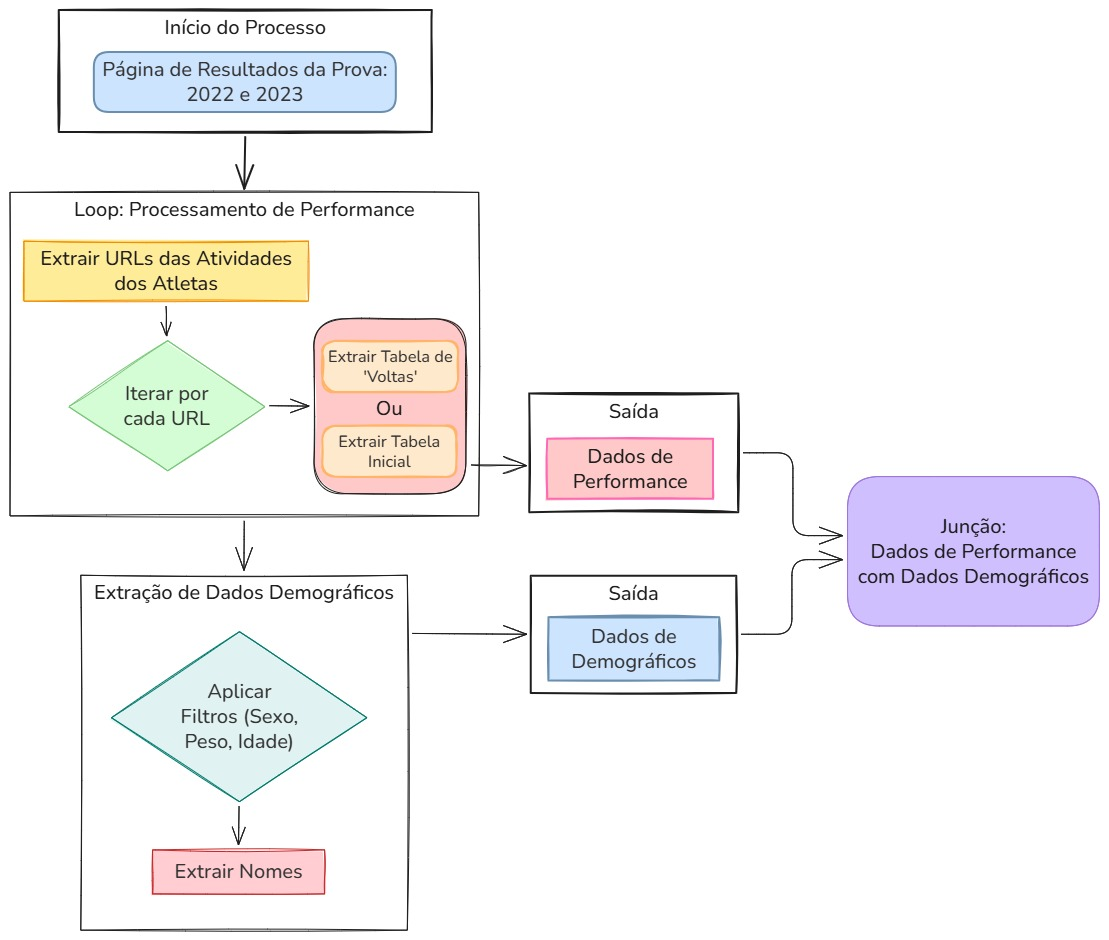
\includegraphics[width=0.7\textwidth]{Imagens/fluxo_webscraping.png}
    \caption{Fluxograma do processo de Web Scraping.}
    \label{fig:fluxograma_scraping}
    \caption*{Fonte: Elaborado pelo autor (2025).}
\end{figure}

\subsection{Limpeza e Estruturação dos Dados}
\label{subsec:limpeza}

Após a extração, foi realizado um rigoroso processo de limpeza e estruturação:
\begin{enumerate}
    \item \textbf{Unificação e Junção:} Os dados de performance dos atletas foram unidos (\emph{join}) aos dados padronizados do percurso (obtidos via GPX) pela coluna indicativa do quilômetro.
    
    \item \textbf{Tratamento de Duplicatas:} Identificou-se que 7 atletas participaram das duas edições da prova. Para garantir a independência das observações, foi mantida apenas a primeira participação de cada um, resultando em 166 atletas únicos nesta fase.
    
    \item \textbf{Padronização de Variáveis:} As colunas de `Tempo` e `Ritmo`, que se apresentavam em formatos distintos, foram unificadas e convertidas para uma unidade padrão de segundos.
    
    \item \textbf{Tratamento de Valores Ausentes:} A estratégia de tratamento de dados faltantes foi definida conforme a variável:
    \begin{itemize}
        \item \textbf{Frequência Cardíaca:} Dada a alta proporção de valores ausentes (superior a 70\%), indicando que a maioria dos atletas não utilizou ou não compartilhou dados de um monitor cardíaco, a variável foi removida do conjunto de dados para evitar a introdução de viés por meio de imputações complexas e pouco confiáveis.
        \item \textbf{Faixa de Peso:} Com aproximadamente 12,44\% de ausência, optou-se por tratar a ausência como uma informação em si. Foi criada a categoria ``Não Informado'', permitindo que o modelo analise se a própria decisão de não informar o peso está associada ao desempenho.
        \item \textbf{Sexo e Faixa Etária:} Com percentuais de ausência baixos (inferiores a 10\%), aplicou-se a técnica de exclusão \textit{listwise}. Esta abordagem foi considerada apropriada sob a suposição de que os dados eram ausentes completamente ao acaso (MCAR, \textit{Missing Completely at Random}), e que a remoção de um pequeno número de observações não introduziria um viés significativo na amostra final \citep[para uma discussão, ver][]{rubin1976}.
    \end{itemize}
\end{enumerate}
Ao final deste processo, consolidou-se um conjunto de dados final, limpo e estruturado no formato \emph{long}, contendo 109 atletas e 36 observações (quilômetros) para cada um.

\subsection{Agregação dos Dados}
\label{sec:preprocessamento}

Para transformar os dados granulares em um formato analítico focado no atleta, foi realizado um processo de agregação. Utilizando uma operação de agrupamento (\texttt{groupby}) por identificador de atleta, o conjunto de dados foi consolidado, passando de uma estrutura por quilômetro para uma estrutura em que cada linha representava um único atleta. Nesta etapa, foram criadas as variáveis agregadas fundamentais para a análise:
\begin{itemize}
    \item \textbf{\texttt{Tempo\_Final\_seg}:} Variável dependente principal do estudo, calculada como a soma total do tempo de cada quilômetro percorrido pelo atleta.
    \item \textbf{\texttt{Ritmo\_Medio\_seg}:} A média do tempo, em segundos, por quilômetro.
    \item \textbf{\texttt{Variabilidade\_Ritmo\_std}:} O desvio padrão do tempo por quilômetro, servindo como a principal métrica de consistência do ritmo do atleta ao longo da prova.
\end{itemize}

\section{Engenharia de Variáveis}
\label{sec:engenharia_variaveis_final}

Após feita a coleta de dados, assim como seu tratamento, foi realizado a etapa crucial da análise que consistiu na elaboração de novas métricas para capturar nuances da estratégia de prova e da performance dos atletas em diferentes terrenos. 

\subsection{Variáveis de Estratégia de Prova (\textit{Splits})}

Para analisar a distribuição de esforço, a prova foi dividida em duas metades: "Primeira Metade" (quilômetros 1-18) e "Segunda Metade" (quilômetros 19-36). A partir dessa segmentação, foram criadas as variáveis \texttt{Ritmo\_Medio\_Primeira\_Metade} e \texttt{Ritmo\_Medio\_Segunda\_Metade}.

Para uma comparação mais robusta da variação de ritmo, foi criada a variável \texttt{diff\_relativa\_segunda\_primeira\_parte}. A justificativa para o uso de uma métrica relativa, em vez de uma diferença absoluta, reside no fato de que uma mesma variação de tempo (e.g., 30 segundos) possui significados distintos para um atleta de elite e um amador. A normalização pelo ritmo médio do próprio atleta gera uma medida de eficiência de \emph{pacing} mais justa e comparável entre corredores de diferentes níveis de habilidade.

\subsection{Variáveis Baseadas em Terreno (Altimetria)}

Para isolar o desempenho em diferentes inclinações, cada quilômetro do percurso foi classificado como "SUBIDA", "DESCIDA", "PLANO" ou "MISTO". Essa classificação foi realizada por uma função customizada (\texttt{Sob\_Desc}) baseada em regras sobre o desnível positivo e negativo de cada trecho. A partir dessa categorização, foram calculadas as variáveis de ritmo médio para cada tipo de terreno, como \texttt{Ritmo\_Medio\_SUBIDA} e \texttt{Ritmo\_Medio\_DESCIDA}.

\subsection{Índices de Performance Relativa}

Visando quantificar a especialização técnica dos atletas, foram desenvolvidos índices normalizados que comparam o desempenho em terrenos específicos com o desempenho geral do próprio indivíduo.
\begin{itemize}
    \item \textbf{\texttt{indice\_subida}:} Mede o quão mais lento um atleta é na subida em comparação com sua própria média geral.
    \item \textbf{\texttt{indice\_descida}:} Mede o quão mais rápido um atleta é na descida em comparação com sua média geral.
    \item \textbf{\texttt{indice\_descida\_vs\_subida}:} Compara diretamente a performance nos dois terrenos-chave, servindo como uma métrica da capacidade de aceleração relativa do atleta em descidas versus subidas.
\end{itemize}

% Adicione este texto no final da Seção 4.5 (Engenharia de Variáveis)
Ao término de todas as etapas de tratamento e engenharia, consolidou-se o conjunto de dados final a ser utilizado nas análises estatísticas subsequentes. A estrutura desta base de dados, em que cada observação corresponde a um atleta único, é detalhada na Tabela \ref{tab:dicionario_variaveis}, que descreve cada variável, seu tipo e sua respectiva unidade de medida.

% Comando para aumentar o espaçamento vertical das linhas
\renewcommand{\arraystretch}{1.5}

\begin{longtable}{ L{0.23\textwidth} L{0.47\textwidth} C{0.15\textwidth} C{0.1\textwidth} }
\caption{Dicionário de variáveis do conjunto de dados final.}
\label{tab:dicionario_variaveis} \\
\toprule
\textbf{Variável} & \textbf{Descrição} & \textbf{Tipo} & \textbf{Unidade} \\
\midrule
\endfirsthead
\multicolumn{4}{c}%
{{\bfseries \tablename\ \thetable{} -- continuação}} \\
\toprule
\textbf{Variável} & \textbf{Descrição} & \textbf{Tipo} & \textbf{Unidade} \\
\midrule
\endhead
\bottomrule
\multicolumn{4}{r}{{\textit{Continua na próxima página}}} \\
\endfoot
\bottomrule
\endlastfoot

% --- DADOS DEMOGRÁFICOS E DE IDENTIFICAÇÃO ---
\multicolumn{4}{l}{\textit{Variáveis de Identificação e Demográficas}} \\
\midrule
\texttt{Nome Atleta} & Identificador único textual para cada atleta. & Categórica & Adim. \\
\midrule

% --- VARIÁVEIS RESPOSTA E DE DESEMPENHO GERAL ---
\multicolumn{4}{l}{\textit{Variáveis Resposta e de Desempenho Geral}} \\
\midrule
\texttt{Tempo\_Final\_seg} & Tempo total para completar a prova. Variável resposta principal. & Quant. \newline Contínua & segundos \\
\texttt{Ritmo\_Medio\_seg} & Ritmo (pace) médio do atleta durante toda a prova. & Quant. \newline Contínua & seg/km \\
\texttt{Variabilidade\_\allowbreak Ritmo\_\allowbreak std} & Desvio padrão do ritmo do atleta nos 36km. Métrica de consistência. & Quant. \newline Contínua & segundos \\
\midrule

% --- VARIÁVEIS DE ESTRATÉGIA DE PROVA (PACING) ---
\multicolumn{4}{l}{\textit{Variáveis de Estratégia de Prova (Pacing)}} \\
\midrule
\texttt{Ritmo\_Medio\_\allowbreak Primeira\_Metade} & Ritmo médio do atleta nos primeiros 18km da prova. & Quant. \newline Contínua & seg/km \\
\texttt{Ritmo\_Medio\_\allowbreak Segunda\_Metade} & Ritmo médio do atleta nos últimos 18km da prova. & Quant. \newline Contínua & seg/km \\
\texttt{diff\_relativa\_...} & Diferença percentual entre o ritmo da segunda e da primeira metade. & Quant. \newline Contínua & \% \\
\texttt{Ritmo\_Medio\_\allowbreak Trecho\_...} & Ritmo médio do atleta em trechos específicos de 5km. & Quant. \newline Contínua & seg/km \\
\midrule

% --- VARIÁVEIS DE DESEMPENHO POR TERRENO ---
\multicolumn{4}{l}{\textit{Variáveis de Desempenho por Terreno}} \\
\midrule
\texttt{Ritmo\_Medio\_\allowbreak SUBIDA} & Ritmo médio do atleta nos trechos classificados como subida. & Quant. \newline Contínua & seg/km \\
\texttt{Ritmo\_Medio\_\allowbreak DESCIDA} & Ritmo médio do atleta nos trechos classificados como descida. & Quant. \newline Contínua & seg/km \\
\texttt{indice\_subida} & Performance relativa em subidas, normalizada pelo ritmo médio geral. & Quant. \newline Contínua & Adim. \\
\texttt{indice\_descida} & Performance relativa em descidas, normalizada pelo ritmo médio geral. & Quant. \newline Contínua & Adim. \\
\texttt{indice\_descida\_\allowbreak vs\_subida} & Razão entre o desempenho em descidas e subidas. & Quant. \newline Contínua & Adim. \\
\bottomrule
\end{longtable}

% É uma boa prática restaurar o valor original do arraystretch depois da tabela
\renewcommand{\arraystretch}{1}

\section{Análise Estatística}
\label{sec:analise_estatistica}

A análise dos dados foi conduzida por meio de um conjunto de técnicas estatísticas, onde a escolha de cada teste foi rigorosamente justificada pelos pressupostos dos dados.

\subsection{Análise Descritiva}
Inicialmente, foi realizada uma análise descritiva com o uso de medidas de tendência central (média, mediana) e dispersão (desvio padrão) para as variáveis quantitativas, e distribuições de frequência para as variáveis categóricas. Visualizações gráficas como histogramas, diagramas de dispersão e \emph{boxplots} foram utilizadas para compreensão visual dos dados e distribuição das variáveis.

\subsection{Testes de Hipóteses}

A comparação do tempo final entre diferentes grupos demográficos foi realizada por meio de testes de hipóteses não-paramétricos. A escolha por essa abordagem foi motivada pela rejeição da hipótese de normalidade da variável resposta \texttt{Tempo\_Final\_seg} nos subgrupos, verificada pelo teste de Shapiro-Wilk para um nível de significância $\alpha = 0.05$. A estatística não-paramétrica é robusta a distribuições não-normais, baseando-se nos postos (\textit{ranks}) das observações em vez de seus valores absolutos \citep{siegel1988}.

\begin{itemize}
    \item \textbf{Comparação entre Sexos:} Para comparar a distribuição do tempo final entre homens e mulheres, utilizou-se o teste de Mann-Whitney U. As hipóteses testadas foram:
    \begin{itemize}
        \item $H_0$: A distribuição do tempo final é a mesma para ambos os sexos.
        \item $H_a$: A distribuição do tempo final é diferente entre os sexos.
    \end{itemize}
    
    \item \textbf{Comparação entre Faixas Etárias e de Peso:} Para comparar o tempo final entre três ou mais grupos independentes (faixas etárias e faixas de peso), empregou-se o teste de Kruskal-Wallis. As hipóteses foram:
    \begin{itemize}
        \item $H_0$: As distribuições do tempo final são as mesmas em todas as faixas (etárias ou de peso).
        \item $H_a$: Pelo menos uma faixa possui uma distribuição de tempo final diferente das demais.
    \end{itemize}
    Em caso de rejeição da hipótese nula, foi aplicado o teste \textit{post-hoc} de Dunn com a correção de Bonferroni para identificar quais pares de grupos apresentavam diferenças estatisticamente significativas, controlando a taxa de erro do Tipo I que inflaciona com múltiplas comparações.
\end{itemize}

\subsection{Análise de Associação}
Para investigar a relação entre a performance (\texttt{Tempo\_Final\_seg}) e a consistência do ritmo (\texttt{Variabilidade\_Ritmo\_std}), utilizou-se o coeficiente de correlação de postos de Spearman ($\rho$). Este método foi escolhido em detrimento da correlação de Pearson devido à não-normalidade das variáveis. Conforme definem \citet{siegel1988}, o teste de Spearman avalia a força e a direção de uma relação monotônica (não necessariamente linear) entre duas variáveis. As hipóteses testadas foram:
\begin{itemize}
    \item $H_0: \rho = 0$ (Não há associação monotônica entre as variáveis).
    \item $H_a: \rho \neq 0$ (Existe uma associação monotônica entre as variáveis).
\end{itemize}

\subsection{Análise de Agrupamento}

Com o objetivo de identificar perfis distintos de corredores ("personas") com base em suas características de prova, foi aplicada a técnica de clusterização não-supervisionada K-Means. O propósito desta análise foi segmentar a amostra em grupos intrinsecamente homogêneos e extrinsecamente heterogêneos, revelando diferentes estratégias e especialidades de desempenho dos atletas.

\subsubsection{Pré-processamento das Variáveis para Clusterização}

O algoritmo K-Means agrupa os dados minimizando a variância intra-cluster, um processo que se baseia fundamentalmente no cálculo de distâncias (tipicamente a distância Euclidiana) entre as observações e os centróides dos clusters. Quando as variáveis de entrada (features) possuem escalas e magnitudes muito diferentes — como, por exemplo, uma variável de tempo em segundos (na casa dos milhares) e um índice de performance (na casa de 0.1 a 0.3) — o cálculo da distância pode ser enviesado. A variável com a maior magnitude iria dominar o cálculo, minimizando ou até anulando a contribuição das outras variáveis para a definição dos grupos.\citep{muller2016}.

Para suavizar este efeito e garantir que todas as variáveis tivessem a mesma importância relativa no processo de agrupamento, foi realizado um pré-processamento de padronização dos dados por meio da técnica \textit{StandardScaler}. Este método transforma cada variável para que ela passe a ter uma média igual a zero e um desvio padrão igual a um. A escolha por essa técnica se justifica pois muitos algoritmos de aprendizado de máquina assumem que as características estão centradas em zero e possuem variância na mesma ordem, evitando que uma variável domine a função objetivo do algoritmo \citep{scikitlearn_preprocessing}. A fórmula para a padronização de cada observação (x) em uma variável é dada por:

\begin{equation}
    z = \frac{x - \mu}{\sigma}
    \label{eq:standardscaler}
\end{equation}

Onde:
\begin{itemize}
    \item $z$ é o valor padronizado (ou z-score);
    \item $x$ é o valor original da observação;
    \item $\mu$ é a média de todos os valores da variável (feature);
    \item $\sigma$ é o desvio padrão de todos os valores da variável.
\end{itemize}

Este passo metodológico foi crucial para assegurar que a formação dos clusters fosse resultado dos padrões nos dados, e não de uma distorção causada pelas diferentes escalas das métricas de desempenho.

\subsubsection{Seleção do Número de Clusters (k)}

A determinação do número ideal de agrupamentos ($k$) é um parâmetro fundamental para o algoritmo K-Means. Para esta finalidade, foi empregado o Método do Cotovelo (\textit{Elbow Method})\citep{thorndike1953}. Este método consiste em executar o algoritmo de clusterização para um intervalo de valores de $k$ (e.g., de 1 a 10) e calcular a soma dos quadrados das distâncias intra-cluster (inércia) para cada valor. O número ótimo de clusters é visualmente identificado no ponto do gráfico onde a adição de um novo cluster não resulta em uma diminuição significativa da inércia, formando um "cotovelo" na curva.


\subsection{Modelagem Preditiva}
Para modelar a relação entre o tempo final e as diversas métricas de desempenho e demográficas, foi ajustado um modelo de Regressão Linear Múltipla, utilizando o método de Estimação por Mínimos Quadrados Ordinários (OLS).

\subsubsection{Especificação do Modelo}
O modelo teórico assume a seguinte forma:
$$ Y = \beta_0 + \beta_1 X_1 + \beta_2 X_2 + \dots + \beta_p X_p + \epsilon $$
Onde $Y$ é a variável dependente (\texttt{Tempo\_Final\_seg}), $X_1, \dots, X_p$ são as variáveis preditoras, $\beta_0, \dots, \beta_p$ são os coeficientes a serem estimados, e $\epsilon$ é o termo de erro aleatório, que se assume seguir uma distribuição normal com média zero e variância constante ($\epsilon \sim N(0, \sigma^2)$).

\subsubsection{Pressupostos do Modelo}
A validade das inferências do modelo OLS depende de um conjunto de pressupostos sobre os erros \citep{montgomery2012}:
\begin{enumerate}
    \item \textbf{Linearidade:} A relação entre as variáveis preditoras e a variável resposta é linear.
    \item \textbf{Independência dos Erros:} Os erros $\epsilon_i$ são independentes entre si.
    \item \textbf{Homocedasticidade:} Os erros possuem variância constante ($\text{Var}(\epsilon_i) = \sigma^2$) para todos os níveis das variáveis preditoras.
    \item \textbf{Normalidade dos Erros:} Os erros são normalmente distribuídos.
\end{enumerate}
A verificação destes pressupostos foi realizada a posteriori, por meio da análise gráfica dos resíduos do modelo ajustado.

\subsubsection{Seleção de Variáveis e Avaliação do Modelo}
Partindo de um modelo inicial com todas as variáveis preditoras potenciais, foi aplicado um processo de seleção de variáveis \textit{backward elimination}. A cada passo, a variável com o maior p-valor acima do nível de significância de 0.05 era removida, buscando-se um modelo final que fosse parcimonioso e interpretável.

Para evitar problemas de multicolinearidade (alta correlação entre preditores), o Fator de Inflação de Variância (VIF) foi calculado para as variáveis do modelo final. Um VIF superior a 5 foi considerado como indicativo de multicolinearidade problemática, levando à remoção da variável em questão.

A qualidade do ajuste do modelo final foi avaliada pelo coeficiente de determinação ajustado ($R^2_{\text{adj}}$), pela significância estatística global do modelo (teste F) e dos coeficientes individuais (teste t), e pela análise de resíduos para validação dos pressupostos.


\section{Softwares Utilizados}

Todas as etapas de coleta, tratamento e análise estatística dos dados foram conduzidas na linguagem de programação Python (versão >= 3.11), com o auxílio de bibliotecas consagradas para manipulação e análise de dados, como Pandas, NumPy, Matplotlib, Seaborn, e para modelagem estatística, como Scikit-learn e Statsmodels.

% --- FIM DO CAPÍTULO DE METODOLOGIA ---